\chapter{Анализ асимптотических свойств периодического решения уравнения Мэки--Гласса}\label{ch:ch1}

В данной главе исследуются релаксационные автоколебания уравнения Мэки--Гласса в предположении, что показатель степени в знаменателе нелинейности --- большой параметр. Рассматривается случай, в котором предельное релейное уравнение, возникающее при устремлении большого параметра к бесконечности, имеет периодическое решение с наименьшим числом переключений на периоде. Для данного случая доказывается существование периодического решения уравнения Мэки--Гласса, асимптотически близкого периодическому решению предельного уравнения.

В первой части главы явно описывается решение предельного уравнения и ограничения на его параметры. Во второй части доказывается асимптотическая (при $\gamma \to +\infty$) сходимость решения уравнения Мэки--Гласса к решению предельного уравнения.

\section{Предельное уравнение Мэки--Гласса}\label{sec:ch1/sec1}

\subsection{Постановка задачи}

Объектом исследования будет уравнение Мэки--Гласса 
\cite{Mackey1977, Glass1988}
\begin{equation}
\label{eq:MG}
\dot{v}=-b v+\frac{a \theta^{\gamma} v(t-\tau)}{\theta^{\gamma}+v^{\gamma}(t-\tau)}.
\end{equation}
Здесь $v=v(t) > 0$ --- скалярная функция, $a, b, \theta, \tau, \gamma$ --- положительные параметры. Параметр $\tau$ --- запаздывание по времени, параметр $\gamma$ определяет форму нелинейности.

После перенормировки параметров и времени
\begin{equation}
\label{eq:substitutions_v}
v(t) = \theta u\Big(\frac{t}{\tau}\Big),\, \beta = b\tau,\, \alpha=a\tau, \, t \mapsto \frac{t}{\tau}
\end{equation}
уравнение \eqref{eq:MG} примет форму
\begin{equation}
\label{eq:MG_norm}
    \dot{u}=-\beta u+\frac{\alpha u(t-1)}{1+(u(t-1))^\gamma}, \text{ где } \alpha > 0, \beta > 0.
\end{equation}

Докажем, что при $\beta \geq \alpha$ положительных периодических решений уравнения \eqref{eq:MG_norm} не существует. Воспользуемся результатом, доказанным в \cite[Proposition 3.1]{Roest2007}.

\begin{definition}
Функцию $f$ назовём унимодальной, если $f(\xi) \geq 0$ при всех $\xi \geq 0$, $f(0) = 0$, и существует единственная точка $\xi_0 > 0$ такая, что $f'(\xi) > 0$ при $0 \leq \xi < \xi_0$ и $f'(\xi) < 0$ при $\xi > \xi_0$, более того, $f''(\xi) < 0$ при $0 \leq \xi \leq \xi_0$ и $\lim\limits_{\xi \to +\infty} f(\xi) = 0$.
\end{definition}

\begin{proposition}
\label{prop:unimodal}
Уравнение $\dot{u}(t) = -\mu u(t) + f(u(t - \tau))$, $\mu > 0$, где функция обратной связи $f$ унимодальна и $f'(0) \leq \mu$, для любого $\tau > 0$ имеет глобально притягивающую неподвижную точку $u^* \equiv 0$ \cite{Roest2007}.
\end{proposition}
% \begin{proof}
% Из условия унимодальности и $f'(0) \leq \mu$ следует, что $\mu \xi_0 > f(\xi_0) \geq f(\xi)$ для всех $\xi \geq 0$.
% 
% Пусть $u(t)$ --- решение, и $u(t_0) \leq \xi_0$ для некоторого $t_0 > 0$, тогда $u(t) \leq \xi_0$ при всех $t > t_0$. Действительно, если это не так, то найдётся момент $t_1 > t_0$ такой, что $u(t_1) = \xi_0$ и $\dot{u(t_1)} \geq 0$. Но $\dot{u(t_1)} = -\mu \xi_0 + f(x(t_1 - \tau)) < 0$, противоречие. Следовательно, множество $[0, \xi_0]$ положительно инвариантно.
% 
% Докажем, что любое положительное решение попадёт в интервал $[0, \xi_0]$. Предположим противное: пусть найдётся момент $t_2$ такой, что при $t > t_2$ верно $u(t) > \xi_0$. Пусть $\Delta_0 = \mu \xi_0 - f(\xi_0) > 0$. Тогда при $t > t_2 + \tau$ верно $\dot{x}(t) < -\Delta_0$ и, следовательно, $x(t) \to -\infty$ при $t \to +\infty$. Противоречие.
% 
% %% РАЗОБРАТЬСЯ И ДОПИСАТЬ.
% \end{proof}

Функция $f(\xi) = \dfrac{\alpha \xi}{1 + \xi^{\gamma}}$ унимодальна, что устанавливается элементарной проверкой. Поскольку $f'(0) = \alpha$, по утверждению \eqref{prop:unimodal} при $\beta \geq \alpha$ функция $u^* \equiv 0$ является глобально притягивающей неподвижной точкой уравнения \eqref{eq:MG_norm}, следовательно, решение уравнения не является периодическим.

В дальнейшем будем считать, что $\alpha > \beta$.

Будем исследовать уравнение \eqref{eq:MG_norm} при больших значениях параметра $\gamma$. Для удобства последующего анализа перейдём к логарифмической шкале. Дальнейший план характерен для уравнений с большим параметром (см., например, \cite{Kolesov2010}): мы рассмотрим предельное при $\gamma\to+\infty$ уравнение и найдём его периодическое решение. Затем будем доказывать наличие периодического режима, близкого к предельному. С этой целью найдём асимптотические формулы решения и докажем теорему о существовании цикла исходного уравнения.

Сделаем в \eqref{eq:MG_norm} экспоненциальную замену $u=e^x$. Данная замена корректна, поскольку $u(t) > 0$. Получим уравнение относительно новой неизвестной $x$:
\begin{equation}
    \label{eq:MG_x}
    \dot{x}=-\beta+\alpha\frac{e^{x(t-1)-x}}{1+e^{\gamma x(t-1)}}.
\end{equation}

\subsection{Предельное релейное уравнение}
При устремлении параметра $\gamma$ к бесконечности получаем следующий предельный для \eqref{eq:MG_x} объект:
\begin{equation}
    \label{eq:MG_rele}
    \dot{x}=-\beta + \alpha \exp({x(t-1)-x})H(\exp({x(t-1)})).
\end{equation}
В правой части релейная функция $H(u)$, которая является предельной для сигмоиды:
\begin{equation}
    \label{eq:H}
    H(u)=\lim\limits_{\gamma\to +\infty}\frac{1}{1+u^{\gamma}}=
    \begin{cases}
        0, & u > 1,\\
        \frac{1}{2}, & u = 1,\\
        1, & u < 1.
    \end{cases}
\end{equation}

\subsection{Множество начальных функций}
Зафиксируем положительные параметры $x_0, p, q$ такие, что $p < q$. В качестве множества начальных функций для уравнений \eqref{eq:MG_x} и \eqref{eq:MG_rele} возьмем множество
\begin{equation}
    \label{eq:init_set}
    S=\{\varphi\in С[-1,0]: 0 < p \leqslant \varphi(t)\leqslant q \text{ при } t\in[-1,0],\ \varphi(0)=x_0\}.
\end{equation}
Это множество непрерывных положительных ограниченных функций на отрезке длины запаздывания, имеющих фиксированное значение $x_0$ в нуле.

\subsection{Решение релейного уравнения}
Введём обозначения:
\begin{equation}
    \label{eq:t0:ch1}
    t_0 = \frac{x_0}{\beta} + 1,
\end{equation}
\begin{equation}
    \label{eq:T}
    T = \frac{1}{\beta} \ln\left(\frac{1}{2}\alpha^2e^{2\beta}(t_1 - t_0 - 1)^2 + \alpha e^{\beta}(t_1 - t_0) + 1\right),
\end{equation}
где $t_1$ --- корень уравнения 
\begin{equation}
    \label{eq:t1_cond_exp}
    e^{\beta (t - t_0)} - \alpha e^{\beta} (t - t_0 - 1) - 1 = 0,
\end{equation}
\begin{equation}
    \label{eq:t2_period}
    t_2 = t_0 + T.
\end{equation}

Справедливо следующее утверждение.

\begin{theorem}[О решении релейного уравнения]\label{thm:relay}
Пусть параметры $\alpha,\beta>0$ удовлетворяют условиям
%
\begin{equation}
    \label{eq:cond_alpha1}
	\begin{cases}
    \alpha > -\dfrac{\beta e^{-\beta}}{W(-e^{-\beta - 1})} & \text{ при } \beta \geq \tilde{\beta},\\
	\alpha > e^{\beta} - e^{-\beta} & \text{ при } 0 < \beta < \tilde{\beta},
	\end{cases}
\end{equation}
где $\tilde{\beta} = 1 + \frac{1}{2} W(-2 e^{-2})$, $W$ --- функция Ламберта, т.~е. обратная к функции $t \mapsto te^t$, рассматриваемой при $t \in [-1; +\infty)$,
\begin{equation}
    \label{eq:cond_alpha2}
    \alpha > \dfrac{e^{\beta(t_1 - t_0 + 1)} - 1}{e^{\beta}(t_1 - t_0)}.
\end{equation}
%
Тогда уравнение \eqref{eq:MG_rele} с начальной функцией из множества \eqref{eq:init_set} имеет $T$~--~периодическое решение
\small
\begin{equation}
    \label{eq:sol_x*}
x^*(t)= 
\begin{cases}
    x_0-\beta t, & t\in[0,t_0],\\
    x_0-\beta t +\ln(\alpha e^{\beta}(t-t_0)+1), & t\in[t_0,t_0+1],\\
    x_0-\beta t + \ln(\frac{\alpha^2}{2}e^{2\beta}(t-t_0-1)^2+\alpha e^{\beta}(t-t_0)+1), & t\in[t_0+1,t_1],\\
    x_0-\beta t + \ln(\frac{\alpha^2}{2}e^{2\beta}(t_1-t_0-1)^2+\alpha e^{\beta}(t_1-t_0)+1), & t\in[t_1,t_2].
\end{cases}
\end{equation}
\normalsize
\end{theorem}

Изображение цикла \eqref{eq:sol_x*} приведено на рисунке \ref{fig:x_star}.

\begin{figure}
\centering
  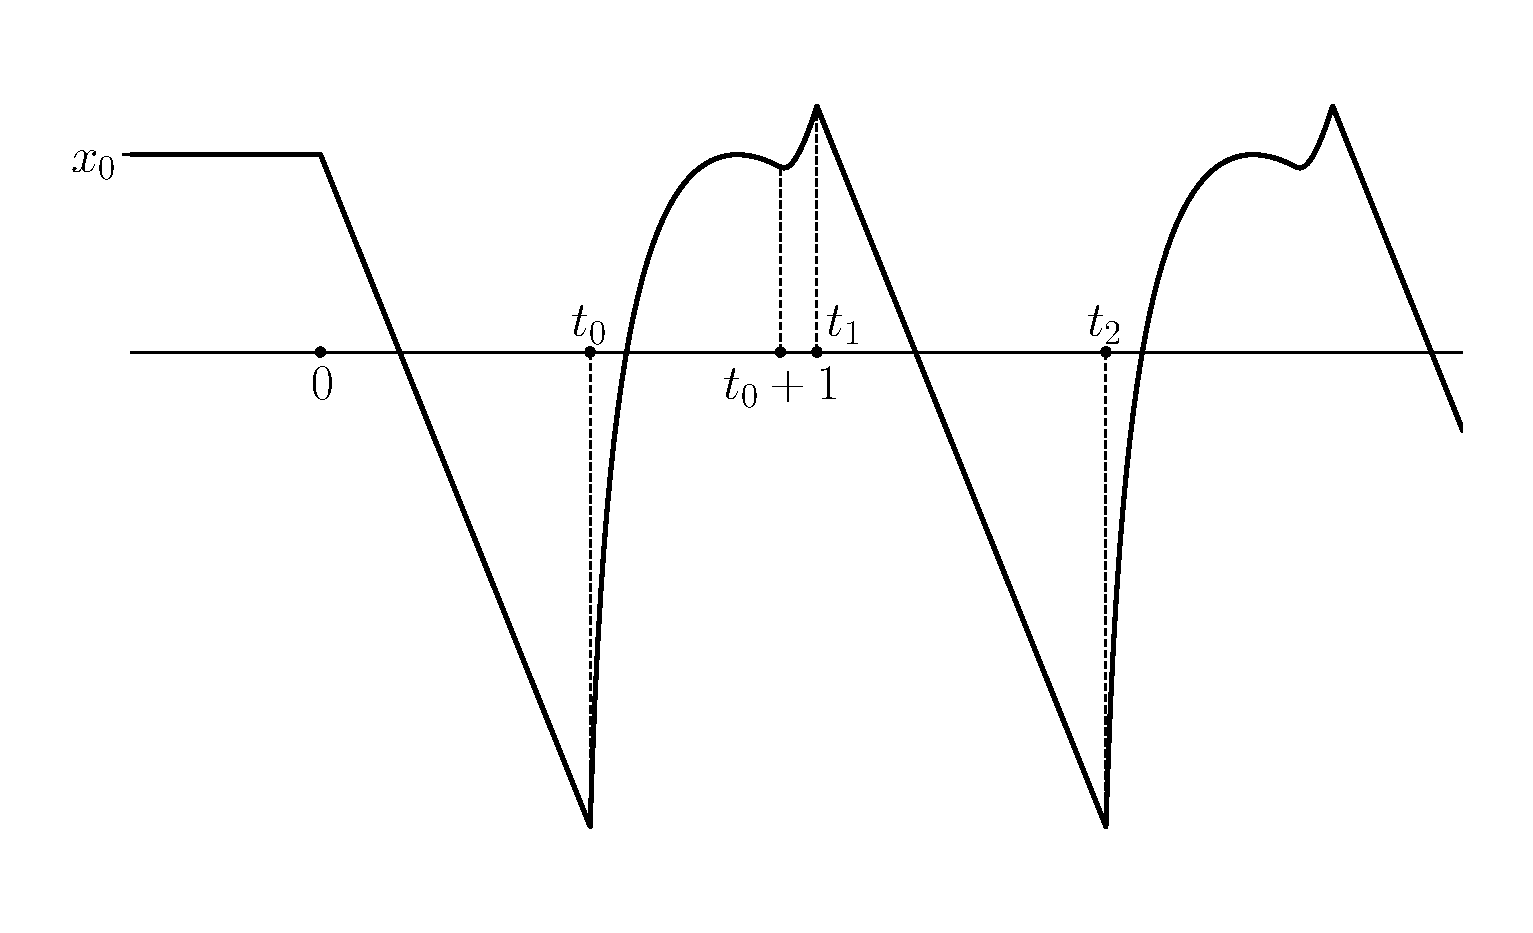
\includegraphics[width=0.7\textwidth]{x_star.eps}
  \captionof{figure}{Периодическое решение $x^{*}(t)$ уравнения \eqref{eq:MG_rele}.}
  \label{fig:x_star}
\end{figure}


\subsection{Доказательство теоремы о решении релейного уравнения}

Решение уравнения \eqref{eq:MG_rele} строится методом шагов.

Если $t \in [0, 1]$, то $x(t - 1) = \phi(t - 1) > 0$, следовательно $x(t)$ отыскивается из начальной задачи Коши
\begin{equation}
    \dot{x} = -\beta, \quad x|_{t = 0} = x_0,
\end{equation}
откуда $x(t) = x_0 - \beta t$. Аналитический вид решения сохраняется до точки $t_0$, поскольку в этой точке величина $x(t - 1)$ меняет знак.

На промежутке $t \in [t_0, t_0 + 1]$ величина $x(t - 1)$ отрицательна, поэтому решение отыскивается из задачи Коши

\begin{equation}
    \dot{x} = -\beta + \alpha\exp(x_0 - \beta(t - 1) - x), \quad x|_{t = t_0} = -\beta,
\end{equation}
откуда находим
\begin{equation}
    x(t) = x_0-\beta t +\ln(\alpha e^{\beta}(t-t_0)+1).
\end{equation}

Следующее изменение аналитического вида решения происходит либо при $t = t_0 + 2$ (в этот момент аргумент функции $x(t - 1)$ выходит из отрезка $[t_0, t_0 + 1]$), либо в точке, где $x(t - 1) = 0$, и величина $x(t - 1)$ второй раз меняет знак.

Проверим, что при ограничении \eqref{eq:cond_alpha1} выполнен второй случай, т.е. корень уравнения
\begin{equation}
\label{eq:t1_eq}
    x_0-\beta (t - 1) +\ln(\alpha e^{\beta}(t - t_0 - 1) + 1) = 0
\end{equation}
существует и лежит на промежутке $(t_0 + 1, t_0 + 2)$.

В \eqref{eq:t1_eq} обозначим $s = t - t_0$ и заменим $x_0 = \beta(t_0 - 1)$, получим
$$-\beta s + \ln(\alpha e^{\beta} (s - 1) + 1) = 0$$
%
или, эквивалентно,
%
\begin{equation}
\label{eq:t1_eq2}
e^{\beta s} - \alpha e^{\beta} (s - 1) - 1 = 0.
\end{equation}
Нужно показать, что при условии \eqref{eq:cond_alpha1} существует корень этого уравнения на промежутке $(1, 2)$.

Обозначим левую часть равенства \eqref{eq:t1_eq2} как $F(s) = e^{\beta s} - \alpha e^{\beta} (s - 1) - 1$. Исследуем функцию $F$:
%
\[
F'(s) = \beta e^{\beta s} - \alpha e^{\beta}, \quad F''(s) = \beta^2 e^{\beta s}.
\]
%
Поскольку $F''(s) > 0$, функция $F$ выпукла. Найдём точку минимума $s_{\min}$ из уравнения $F'(s) = 0$.
\[
\beta e^{\beta s} - \alpha e^{\beta} = 0 \Leftrightarrow s = 1 + \frac{1}{\beta}\ln\frac{\alpha}{\beta}.
\]
%
Поскольку при $\alpha > \beta$ верно $s_{\min} > 1$ и $F(1) = e^{\beta} - 1 > 0$, корень $s = s_* > 1$ существует тогда и только тогда, когда $F(s_{\min}) \leqslant 0$. Выразим $\alpha$ из этого условия.
%
\[
F(s_{\min}) = \frac{\alpha}{\beta}e^{\beta} - \frac{\alpha}{\beta}e^\beta\ln\frac{\alpha}{\beta} - 1 \leq 0 \Leftrightarrow \frac{\alpha}{\beta}e^{\beta}\left(1 + \ln\frac{\beta}{\alpha}\right) < 1.
\]

% Обозначим левую часть равенства \eqref{eq:t1_eq2} как $F(s)$; $F''(s) > 0$, поэтому $F(s)$ выпукла. Минимум $F(s)$ достигается в точке $s_{\min} = 1 + \frac{1}{\beta}\ln\frac{\alpha}{\beta}$. Поскольку $s_{\min} > 1$ и $F(1) = e^{\beta} - 1 > 0$, корень $s = s_* > 1$ существует тогда и только тогда, когда $F(s_{\min}) \leqslant 0$; это эквивалентно условию
% $$\alpha \geqslant \dfrac{-\beta e^{-\beta}}{W(-e^{-\beta - 1})}.$$

Условие $s_* < 2$ выполняется, если $F(2) < 0$ или $s_{\min} < 2$, что эквивалентно (в первом случае) $\alpha > e^{\beta} - e^{-\beta}$ или (во втором случае) $\alpha < \beta e^{\beta}$.

Совокупность приведённых условий (с точностью до замены нестрогих неравенств на строгие) эквивалентна \eqref{eq:cond_alpha1}, что показывает следующая лемма.

\begin{lemma}
\label{lm:parameter_constraints:ch1}
Совокупность неравенств 
\[
\begin{cases}
\left[
\begin{array}{ll}
	\alpha > e^{\beta} - e^{-\beta},\\
    \alpha < \beta e^{\beta},
\end{array}
\right.\\
\frac{\alpha}{\beta}e^{\beta}\left(1 + \ln\frac{\beta}{\alpha}\right) < 1
\end{cases}
\]
эквивалентна условиям \eqref{eq:cond_alpha1}.
\end{lemma}
\begin{proof}
Элементарными преобразованиями получаем: 
\[
e^{\beta} - e^{-\beta} = \beta e^{\beta} \Leftrightarrow (2\beta - 2) e^{2\beta - 2} = -2e^{-2}.
\]
Для отображения $t \mapsto te^t$ каждая точка из интервала $(-1, 0)$ имеет ровно два прообраза, следовательно, возможны две ситуации: $2\beta - 2 = -2$, откуда $\beta = 0$, и $2\beta - 2 = W(-2e^{-2})$, откуда $\beta = \tilde{\beta}$.

Также заметим, что $(e^{\beta} - e^{-\beta})'|_{\beta = 0} > (\beta e^{\beta})'|_{\beta = 0}$, поэтому на промежутке $(0, \tilde{\beta})$ верно неравенство $e^{\beta} - e^{-\beta} > \beta e^{\beta}$. На промежутке $(\tilde{\beta}, +\infty)$ верно обратное неравенство из асимптотических соображений при $\beta \to +\infty$.

Теперь явно выразим $\alpha$ из третьего неравенства в условии леммы.
\begin{equation*}
\frac{\alpha}{\beta}e^{\beta}\left(\ln\frac{\beta}{\alpha} + 1\right) < 1\ \Leftrightarrow\ 1 + \ln\dfrac{\beta}{\alpha} < \dfrac{\beta e^{-\beta}}{\alpha}.
\end{equation*}

Возьмём экспоненту от обеих частей:
\begin{equation*}
\dfrac{e\beta}{\alpha} < \exp\dfrac{\beta e^{-\beta}}{\alpha}\ \Leftrightarrow\ \dfrac{-\beta e^{-\beta}}{\alpha}\exp \dfrac{-\beta e^{-\beta}}{\alpha} > -e^{-\beta - 1}\ \Leftrightarrow
\end{equation*}

\begin{align}
\label{eq:step3_cond1_expanded:ch1}
\left[
\begin{array}{ll}
    -\frac{\beta e^{-\beta}}{\alpha} > W(-e^{-\beta - 1}),\\
    -\frac{\beta e^{-\beta}}{\alpha} < W_{-1}(-e^{-\beta - 1}).
\end{array}
\right.
\end{align}
%
где $W_{-1}(x)$ --- ветвь функции Ламберта, принимающая значения из промежутка $(-\infty; -1]$.

Однако, второе неравенство соответствует случаю $\dfrac{-\beta e^{-\beta}}{\alpha} < -1$, поскольку $W_{-1}(x) < -1$. Тогда
\[
\alpha < \beta e^{-\beta} < \beta,
\]
что противоречит условию $\alpha > \beta$.

Значит, совокупность неравенств \eqref{eq:step3_cond1_expanded:ch1} заменяется на единственное неравенство
\[
    -\frac{\beta e^{-\beta}}{\alpha} > W(-e^{-\beta - 1}) \Leftrightarrow \alpha > -\dfrac{\beta e^{\beta}}{W(-e^{-\beta - 1})}.
\]
%
Знак неравенства меняется, поскольку $W(-e^{-\beta - 1}) < 0$.

Докажем, что $-\dfrac{\beta e^{-\beta}}{W(-e^{-\beta - 1})} > \beta e^{\beta}$ тогда и только тогда, когда $0 < \beta < \tilde{\beta}$.
%
\[
-\dfrac{\beta e^{\beta}}{W(-e^{-\beta - 1})} > \beta e^{\beta} \Leftrightarrow W(-e^{-\beta - 1}) > -e^{-2\beta} \Leftrightarrow -e^{-\beta - 1} > -e^{-2\beta} \exp(-e^{-2\beta}) \Leftrightarrow
\]
%
\[
\Leftrightarrow e^{\beta - 1} < \exp(-e^{-2\beta}) \Leftrightarrow \beta - 1 < -e^{-2\beta} \Leftrightarrow \beta e^{\beta} < e^{\beta} - e^{-\beta}.
\]
Последнее неравенство верно при $0 < \beta < \tilde{\beta}$, как было доказано выше.

Докажем, что $-\dfrac{\beta e^{-\beta}}{W(-e^{-\beta - 1})} \leqslant e^{\beta} - e^{-\beta}$.

%% !!TODO: завершить доказательство!
\textbf{Здесь будет завершение доказательства. Оно есть во второй части в более общем случае, может можно сослаться или привести в виде леммы здесь.}

\end{proof}

На отрезке $t \in [t_0 + 1, t_1]$ решение отыскивается из задачи Коши 
%
\begin{multline}
    \dot{x} = -\beta + \alpha\exp\bigg(x_0 - \beta(t - 1) + \ln(\alpha e^{\beta}(t - t_0 - 1) + 1) - x\bigg),\\
    x|_{t = t_0 + 1} = x_0 - \beta (t_0 + 1) +\ln(\alpha e^{\beta} + 1),
\end{multline}
%
откуда находим
\begin{equation}
    x(t) = x_0-\beta t+\ln\left(\frac{\alpha^2}{2}e^{2\beta}(t-t_0-1)^2+\alpha e^{\beta}(t-t_0)+1\right).
\end{equation}
%
При $t > t_1$ величина $x(t - 1)$ становится положительной, поэтому уравнение \eqref{eq:MG_rele} вновь принимает вид $\dot{x} = -\beta$. Пусть $t_2$ --- следующий корень уравнения $x(t - 1) = 0$, а именно
\begin{equation}
\label{eq:t2}
t_2 = 1 + \dfrac{1}{\beta}\ln\left(\frac{\alpha^2}{2}e^{2\beta}(t-t_0-1)^2+\alpha e^{\beta}(t-t_0)+1\right).
\end{equation}

С учётом начальных условий в точке $t_1$, на промежутке $[t_1, t_2]$
\begin{equation}
\label{eq:sol_rele_3}
    x(t) = x_0-\beta t+\ln\left(\frac{\alpha^2}{2}e^{2\beta}(t_1-t_0-1)^2+\alpha e^{\beta}(t_1-t_0)+1\right).
\end{equation}

Отбросим в \eqref{eq:sol_rele_3} квадратичное слагаемое, получим выпуклую вверх функцию $\tilde{x}(t) = -\beta(t - t_0 + 1) + \ln(\alpha e^{\beta} (t - t_0) + 1)$, равную нулю в точке $t_1 - 1$. Тогда $\tilde{x}(t) > 0$ на промежутке $(t_1 - 1, t_1]$, если $\tilde{x}(t_1) > 0$. Выражая из этого неравенства $\alpha$, с учётом $x(t) \geqslant \tilde{x}(t)$ получим условие \eqref{eq:cond_alpha2}.

Пусть $t_2$ --- корень уравнения $x(t - 1) = 0$, больший $t_1$. Поскольку $x(t) > 0$ на промежутке длины не меньше единицы, последующие шаги построения решения будут совпадать с приведёнными выше, и решение $x(t)$ будет периодическим с периодом $T = t_2 - t_0$. Подставляя соответствующие значения из \eqref{eq:t0:ch1} и \eqref{eq:t2}, получаем явное значение периода \eqref{eq:T}.

% Отметим, что при $\alpha > \exp(\beta + e^{-\beta})$ условия теоремы выполняются (в этом можно убедиться явной проверкой условий).
% Расписать подробнее

\subsection{Явные ограничения на параметры уравнения}

Одновременное выполнение условий \eqref{eq:cond_alpha1} и \eqref{eq:cond_alpha2} затруднительно для проверки. Сформулируем достаточное условие, позволяющее легко находить подходящие наборы параметров $\alpha$ и $\beta$.

\begin{theorem}
Пусть параметры $\alpha$, $\beta$ таковы, что $\beta > 0$, $\alpha > \exp(\beta + e^{-\beta})$. Тогда $\alpha$ и $\beta$ удовлетворяют условиям \eqref{eq:cond_alpha1} и \eqref{eq:cond_alpha2}.
\end{theorem}
\begin{proof}
	Поскольку, очевидно, $\exp(\beta + e^{-\beta}) > e^{\beta} - e^{-\beta}$, условие \eqref{eq:cond_alpha1} выполнено.	
	
	%% !!TODO: завершить доказательство!
	\textbf{Здесь будет завершение доказательства. Оно есть во второй части в более общем случае, может можно сослаться или привести в виде леммы здесь.}
	
	
\end{proof}

%%%%%%
%%% ОСНОВНОЙ РАЗДЕЛ ПРО АСИМПТОТИКИ
%%%%%%
\section{Асимптотика уравнения Мэки--Гласса}


%% !!TODO: Здесь пока нет единтвенности. Для доказательства единственности надо написать производную Фреше.
\begin{theorem}
    \label{thm:existence}
Пусть параметры $\alpha > \beta > 0$ удовлетворяют условиям \eqref{eq:cond_alpha1}, \eqref{eq:cond_alpha2}. Тогда существуют такие значения параметров $x_0, p, q$ и такое достаточно большое $\gamma_0$, что при всех $\gamma > \gamma_0$ уравнение \eqref{eq:MG_x} с начальной функцией из множества \eqref{eq:init_set} обладает периодическим решением $x^*_\gamma(t)$ периода $T_\gamma$, которое удовлетворяет предельным равенствам 
\begin{equation}
\label{eq:lim_x*}
	\lim_{\gamma\to+\infty}\max_{0\leqslant t\leqslant T_\gamma}|x_{\gamma}^*(t)-x^*(t)|=0,\quad \lim_{\gamma\to+\infty}T_{\gamma} = T.
\end{equation}
\end{theorem}

\subsection{Общая схема доказательства}
Будем последовательно находить асимптотические формулы решения $x_{\gamma}^*(t)$ уравнения \eqref{eq:MG_x} методом шагов, опираясь на решение $x^*(t)$ релейного уравнения \eqref{eq:MG_rele}. Техника построения асимптотики сходна с описанной в работах \cite{Kolesov2010, Glyzin2013}.

Назовем \textit{точкой излома} функции $x^*(t)$ точку, в которой она имеет разные односторонние производные. Точки излома следует искать среди точек, в которых функция $x^*(t)$ меняет аналитический вид, то есть среди точек $t_0$, $t_0+1$, $t_1$. Однако, в точке $t_0+1$ производные справа и слева совпадают и равны $-\beta+\frac{\alpha e^{\beta}}{\alpha e^{\beta}+1}$, то есть $t_0+1$ не является точкой излома функции $x^*(t)$. Производные в точке $t_0$ справа и слева равны соответственно $-\beta$ и $-\beta+\alpha e^\beta$, в точке $t_1$ они равны $$-\beta+\frac{\alpha^2e^{2\beta}(t_1-t_0-1)+\alpha e^\beta}{\frac{\alpha^2}{2}e^{2\beta}(t_1-t_0-1)^2+\alpha e^{\beta}(t_1-t_0)+1}$$ слева и $-\beta$ справа. 
Таким образом, функция $x^*(t)$ имеет две точки излома: $t_0$ и $t_1$.

Зафиксируем параметр $\nu\in(\frac{1}{2}, 1)$ и введем малый параметр $\sigma$, который следующим образом связан с большим параметром $\gamma$:  
%
\[\sigma=\gamma^{-\nu}.\]
%
Параметр $\sigma$ имеет смысл радиуса малой окрестности точки излома.

На отрезках 
$[0,t_0-\sigma],$ 
$[t_0+\sigma, t_0+1-\sigma],$ 
$[t_0+1-\sigma,t_0+1+\sigma],$ 
$[t_0+1+\sigma,t_1-\sigma],$ 
$[t_1+\sigma,t_2-\sigma]$ 
будем искать решение в виде
%
\begin{equation}
    \label{eq:x*gamma_1}
    x^*_\gamma(t) = x^*(t) + \Delta
\end{equation}
и доказывать малость остатка $\Delta$. Для этого найдем задачу Коши, которой удовлетворяет остаток $\Delta$. С этой целью подставим \eqref{eq:x*gamma_1} в \eqref{eq:MG_x}, в результате чего получим уравнение
%
\begin{equation*}
    \dot{\Delta} = -\beta + \frac{\alpha\exp(x_{\gamma}^*(t - 1) - x^*(t))}{1 + \exp(\gamma x_{\gamma}^*(t - 1))}e^{-\Delta}-\dot{x}^*.
\end{equation*}
%
Обозначим начало рассматриваемого отрезка через $\tilde{t}$, а значение функции $\Delta$ в этой точке --- через $\tilde{\Delta}$. Для того чтобы найти начальное значение, приравняем значение в точке $\tilde{t}$ функции $x_{\gamma}^*(t)$ на предыдущем и текущем шагах:
%
\[x_{\gamma}^*(\tilde{t}-0)=x^*(\tilde{t}+0)+\Delta|_{t=\tilde{t}}.\]
%
Таким образом, $\Delta$ удовлетворяет задаче Коши
\begin{equation}
        \label{eq:task_DeltaAB}
        \dot{\Delta}=A e^{-\Delta} + B,\quad \Delta|_{t=\tilde{t}}=\tilde{\Delta},
\end{equation}
%
\begin{equation}
    \label{AB_eq:x*gamma_1}
\text{где } A = \frac{\alpha\exp(x_{\gamma}^*(t - 1) - x^*(t))}{1+\exp(\gamma x_{\gamma}^*(t - 1))},\, 
B = -\beta-\dot{x}^*,\, 
\tilde{\Delta}=x_{\gamma}^*(\tilde{t} - 0) - x^*(\tilde{t} + 0).
\end{equation}

На отрезках $[t_i - \sigma, t_i + \sigma],$ $i=0, 1,$ будем предполагать, что решение имеет вид
%
\begin{equation}
    \label{eq:x*gamma_2}
    x^*_\gamma(t)=x^*(t_i)+\frac{1}{\gamma}w_i(\tau)|_{\tau=(t-t_i)\gamma}+\Delta.
\end{equation}
%
Здесь $w_i(\tau)$ --- известные, специальным образом выбранные нами функции. Подробнее о них будет написано в следующем пункте. Параметр $\Delta$ --- предстоящий определению остаток, малость которого требуется доказать. Для определения задачи Коши, которой он удовлетворяет, подставим \eqref{eq:x*gamma_2} в \eqref{eq:MG_x} и найдем начальное значение. Получим задачу \eqref{eq:task_DeltaAB} при
\begin{equation}
    \label{AB_eq:x*gamma_2}
    A=\frac{\alpha\exp\big(x_{\gamma}^*(t-1)-x^*(t_i)-\frac{1}{\gamma}w_i(\tau)|_{\tau=(t-t_i)\gamma}\big)}{1+\exp(\gamma x_{\gamma}^*(t-1))},
    \,
    B=-\beta-\frac{dw_i}{d\tau}\Big|_{\tau=(t-t_i)\gamma},
\end{equation}
%
\begin{equation}\label{tilde_eq:x*gamma_2}
    \tilde{t} = t_i - \sigma = t_i - \gamma^{-\nu},\quad \tilde{\Delta}=x_{\gamma}^*(\tilde{t} - 0) - x^*(t_i) -\frac{1}{\gamma} w_i(\tau)|_{\tau = -\gamma^{1 - \nu}}.
\end{equation}
%% !!DONE: проверено.

Получаем, что на каждом из рассматриваемых отрезков, остаток $\Delta$ находится из задачи Коши \eqref{eq:task_DeltaAB}. Докажем вспомогательное утверждение.

\begin{lemma}\label{lm:DeltaAB}
Пусть $\tilde{t} \geqslant 0$, $\tilde{\Delta}$ --- известные вещественные числа, $A = A(t),$ $B = B(t)$ --- непрерывные при $t \geq \tilde{t}$ функции, $A(t) > 0$. Тогда решение задачи Коши \eqref{eq:task_DeltaAB} выражается формулой
	\begin{equation}\label{sol_DeltaAB}
	\Delta = J + \ln\Big(1 + \int\limits_{\tilde{t}}^{t} A(s) e^{-J}\,ds \Big),
	\text{ где } J = \tilde{\Delta} + \int\limits_{\tilde{t}}^{t} B(s)\,ds.
	\end{equation}
\end{lemma}
\begin{proof}
    Замена $e^{\Delta}=\theta$ преобразует задачу \eqref{eq:task_DeltaAB} к виду
	%
    \begin{equation}\label{task_theta}
		\dot{\theta}=A+B\theta,\quad\theta|_{t=\tilde{t}}=e^{\tilde{\Delta}}.
    \end{equation}
	%
    Решение соответствующей однородной задачи $\dot{\theta}=B\theta$, $\theta|_{t=\tilde{t}}=e^{\tilde{\Delta}}$ --- это функция $\theta_*(t)=\exp(\tilde{\Delta}+\int\limits_{\tilde{t}}^{t}B(s)ds).$ Тогда решение задачи \eqref{task_theta} --- это $\theta=\theta_* y$, где $y$ удовлетворяет задаче $\dot{y} = A \theta^{-1}$, $y|_{t=\tilde{t}} = 1$. Отсюда $y = 1 + \int\limits_{\tilde{t}}^{t}A(s)\theta_*^{-1}ds$, следовательно $\theta=\theta_*(1+\int\limits_{\tilde{t}}^{t}A(s)\theta_*^{-1}ds)$.
    Тогда $\Delta=\ln\theta=\ln\theta_*+\ln(1+\int\limits_{\tilde{t}}^{t}A(s)\theta_*^{-1}ds),$ откуда следует формула \eqref{sol_DeltaAB}.
\end{proof}
%%!! DONE: проверено.

Из леммы \eqref{lm:DeltaAB} и формул \eqref{AB_eq:x*gamma_1}, \eqref{AB_eq:x*gamma_2}, \eqref{tilde_eq:x*gamma_2} получаем следствия.
\begin{corollary}\label{corol_Delta_long}
На отрезках $[0, t_0-\sigma],$ $[t_0+\sigma, t_0+1-\sigma],$ $[t_0+1-\sigma, t_0+1+\sigma],$ $[t_0+1+\sigma, t_1-\sigma],$ $[t_1+\sigma,t_2-\sigma],$ где решение имеет вид \eqref{eq:x*gamma_1}, остаток $\Delta$ определяется формулой
\begin{equation}
    \label{Delta}
    \Delta = J + \ln(1 + I),
\end{equation}
где 
\begin{equation}
    \label{I_long}
    I = \int\limits_{\tilde{t}}^{t}\frac{\alpha\exp(x_{\gamma}^*(s-1)+\beta(s-\tilde{t})-x_{\gamma}^*(\tilde{t}))}{1 + \exp(\gamma x_{\gamma}^*(s-1))} ds,
\end{equation}
%
\begin{equation}\label{J_long}
    J = x_{\gamma}^*(\tilde{t}) - x^*(t) - \beta(t - \tilde{t}),
\end{equation}
%
$\tilde{t}$ --- начальная точка рассматриваемого отрезка.
\end{corollary}
%
\begin{proof}
	Подставим в формулу \eqref{sol_DeltaAB} значения $A$ и $B$ из \eqref{AB_eq:x*gamma_1}. Получим $\Delta = J + \ln(1 + I)$, где
\begin{multline*}
	J = \tilde{\Delta} + \int\limits_{\tilde{t}}^{t}(-\beta - \dot{x}^*(s))ds = x_{\gamma}^*(\tilde{t}) - x^*(\tilde{t}) - \beta(t - \tilde{t}) - x^*(t) + x^*(\tilde{t}) =\\= x_{\gamma}^*(\tilde{t}) - x^*(t) - \beta(t - \tilde{t}),
\end{multline*}
\[
	I = \int\limits_{\tilde{t}}^{t} A e^{-J} \, ds = \int\limits_{\tilde{t}}^{t}\frac{\alpha\exp(x_{\gamma}^*(s-1)+\beta(s-\tilde{t})-x_{\gamma}^*(\tilde{t}))}{1 + \exp(\gamma x_{\gamma}^*(s-1))} ds.
\]
\end{proof}
%
\begin{corollary}\label{corol_Delta_short}
На отрезках $[t_i-\sigma,t_i+\sigma]$, $i=0, 1$, где решение имеет вид \eqref{eq:x*gamma_2}, остаток $\Delta$ определяется формулой \eqref{Delta} при
 \begin{equation}
    \label{I_point}
   I=\int\limits_{t_i-\sigma}^{t}\frac{\alpha\exp\big(x_{\gamma}^*(s-1)+\beta(s-t_i+\sigma)-x_{\gamma}^*(t_i-\sigma)\big)}{1+\exp(\gamma x_{\gamma}^*(s-1))}ds,
\end{equation}
%
\begin{equation}
    \label{J_point}
    J=x_{\gamma}^*(t_i - \sigma) - x^*(t_i) - \beta(t-t_i+\sigma) - \frac{1}{\gamma} w_i(\tau)|_{\tau=(t-t_i)\gamma}.
\end{equation}
\end{corollary}
%
\begin{proof}
	Выражая $\tilde{\Delta} = \Delta|_{t = t_i - \sigma}$ из \eqref{eq:x*gamma_2}, получаем
\[
	\tilde{\Delta} = x^*_{\gamma}(t_i - \sigma) - x^*(t_i) - \frac{1}{\gamma} w_i(\tau)|_{\tau = -\gamma^{1-\nu}}.
\]
Пусть $\tilde{t} = t_i - \sigma$. Учитывая $\frac{d}{d\tau} w_i(\tau)|_{\tau = \gamma(t - t_i)} = \frac{d}{dt} \left(\frac{1}{\gamma}w_i(\tau)\right)\big|_{\tau = \gamma(t - t_i)}$, в формуле \eqref{sol_DeltaAB} получаем
\begin{multline*}
	J = \tilde{\Delta} + \int\limits_{\tilde{t}}^{t} B(s)\,ds = \tilde{\Delta} + \int\limits_{\tilde{t}}^{t} -\beta - \frac{d}{ds} \left(\frac{1}{\gamma}w_i(\tau)\right)\big|_{\tau = \gamma(s - t_i)} \,ds =\\= x^*_{\gamma}(t_i - \sigma) - x^*(t_i) - \frac{1}{\gamma} w_i(\tau)|_{\tau = -\gamma^{1-\nu}} - \frac{1}{\gamma}w_i(\tau)|_{\tau = \gamma(t - t_i)} + \frac{1}{\gamma}w_i(\tau)_{\tau = -\gamma^{1 - \nu}} = \\
	= x^*_{\gamma}(t_i - \sigma) - x^*(t_i) - \beta(t - t_i - \sigma) - \frac{1}{\gamma} w_i(\tau)|_{\tau = \gamma(t - t_i)}.
\end{multline*}
%
По лемме \ref{lm:DeltaAB} получаем, что остаток имеет вид $\Delta = J + \ln(1 + I)$, где 
\[
I = \int\limits_{\tilde{t}}^{t}A(s) e^{-J} ds = \int\limits_{t_i-\sigma}^{t}\frac{\alpha\exp\big(x_{\gamma}^*(s-1)+\beta(s-t_i+\sigma)-x_{\gamma}^*(t_i-\sigma)\big)}{1+\exp(\gamma x_{\gamma}^*(s-1))}ds.
\]
\end{proof}
%% !!DONE: проверено.
%% !!TODO: добавить развёрнутые выкладки.
%
Отметим, что $x_{\gamma}^*(\tilde{t})$ и $x_{\gamma}^*(t_i-\sigma)$ в следствиях \ref{corol_Delta_long} и \ref{corol_Delta_short} определяются формулами, полученными на предыдущих шагах.


\subsection{Асимптотическое поведение в окрестности точек излома}

Как было написано выше, для описания асимптотического поведения решения уравнения \eqref{eq:MG_x} в окрестности точек излома введем специальные функции:
%
\begin{equation}
    \label{eq:w0}
    w_0(\tau)=-\beta \tau+\frac{\alpha e^\beta}{\beta}\ln(e^{\beta\tau}+1),
\end{equation}
%
\small
\begin{multline}
    \label{eq:w1}
    w_1(\tau)=-\beta\tau-\frac{\alpha e^\beta(\alpha e^\beta(t_1-t_0-1)+1)^2}{(-\beta(\alpha e^\beta(t_1-t_0-1)+1)+\alpha e^\beta)(\frac{\alpha^2}{2}e^{2\beta}(t_1-t_0-1)^2+\alpha e^{\beta}(t_1-t_0)+1))}\times
    \\
    \times\ln\Bigg(\exp\Big(\beta\tau-\frac{\alpha e^\beta\tau}{\alpha e^\beta(t_1-t_0-1)+1}\Big)+1\Bigg).
\end{multline}
\normalsize

Сформулируем и докажем утверждение, описывающее асимптотическое поведение введенных функций \eqref{eq:w0}, \eqref{eq:w1} при $\tau\to-\infty$ и $\tau\to+\infty$.
%
\begin{lemma}\label{lm:w_asymp}
\begin{equation}
    \label{eq:w0_asymp-}
    w_0(\tau)=-\beta \tau+O(e^{\beta\tau}) \text{ при } \tau\to -\infty,
\end{equation}
%
\begin{equation}
    \label{eq:w0_asymp+}
    w_0(\tau)=(-\beta+\alpha e^\beta) \tau+O(e^{-\beta\tau}) \text{ при } \tau\to +\infty,
\end{equation}
%
\begin{multline}
    \label{eq:w1_asymp-}
    w_1(\tau)=\Big(-\beta+\frac{\alpha e^\beta(\alpha e^\beta(t_1-t_0-1)+1)}{\frac{\alpha^2}{2}e^{2\beta}(t_1-t_0-1)^2+\alpha e^\beta(t_1-t_0)+1}\Big)\tau+
    \\
    +O\Big(\exp\Big(-\beta\tau+\frac{\alpha e^\beta\tau}{\alpha e^\beta(t_1-t_0-1)+1}\Big)\Big)\text{ при } \tau\to -\infty,
\end{multline}
%
\begin{equation}
    \label{eq:w1_asymp+}
    w_1(\tau)=-\beta\tau+O\Big(\exp\Big(\beta\tau-\frac{\alpha e^\beta\tau}{\alpha e^\beta(t_1-t_0-1)+1}\Big)\Big) \text{ при } \tau\to +\infty,
\end{equation}
\end{lemma}